\documentclass[a4paper,11pt]{article}

\usepackage[left=2.5cm,top=2.5cm,right=2.5cm]{geometry}

\usepackage{graphicx, subfigure}
\usepackage{longtable}
\usepackage{url}
\usepackage{moreverb}
\usepackage{float}
\usepackage{placeins}
\usepackage{cite}

\usepackage{framed}
\usepackage{color}
\definecolor{lightgray}{rgb}{0.95,0.95,0.95}
\def\FrameCommand{\colorbox{lightgray}}

\usepackage{sistyle}
\SIunitsep{{\;}}
\SIunitspace{{\,}}

\usepackage[Euler]{upgreek}
\newcommand*{\micro}{\ensureupmath{\upmu}}
\newcommand*{\ohm}{\ensureupmath{\upOmega}}

\usepackage[version=3]{mhchem}

\newcommand{\code}[1]{\texttt{#1}}
\newcommand{\cmd}[1]{\texttt{\color{blue}#1}}

\def\figratio{0.7}

\title{ssh-aerosol}
\date{}
\author{ssh-aerosol user manual and test cases}

\begin{document}

\maketitle

\section*{About}

\begin{itemize}
\item[] {\bf Purpose:} introduction to ssh-aerosol and launching simulations
  for test cases. Very basic post-processing is also
  presented. 
\item[] {\bf Authors:} \\Karine Sartelet, \url{karine.sartelet@enpc.fr};\\
  Youngseob Kim, \url{youngseob.kim@enpc.fr};\\ Zhizhao Wang,
  \url{zhizhao.wang@enpc.fr}; \\Florian Couvidat, \url{florian.couvidat@ineris.fr}.
\item[] {\bf ssh-aerosol version:} 0.7
\end{itemize}

\tableofcontents

\newpage

\section{Introduction}
\addcontentsline{toc}{section}{Introduction}
The ssh-aerosol model is modular and the user can choose the physical and chemical complexity required.
The model is based on the merge of three state-of-the-art models:
\begin{itemize}
\item SCRAM : The Size-Composition Resolved Aerosol Model \cite{zhu2015size} that simulates the dynamics and the mixing state of atmospheric particles. It classifies particles by both composition and size, based on a comprehensive combination of all chemical species and their mass-fraction sections. All three main processes involved in aerosol dynamics (coagulation, condensation/evaporation and nucleation) are included.
\item SOAP: The Secondary Organic Aerosol Processor \cite{couvidat2015secondary} is a thermodynamic model that compute the partitioning of organic compounds. It takes into account several processes involved in the formation of organic aerosol (hygroscopicity, absorption into the aqueous phase of particles, non-ideality and phase separation) and computes the formation of organic aerosol either with a classic equilibrium representation (the partitioning of organic compounds is instantaneous) or with a dynamic representation (where the model solves the dynamic of the condensation/evaporation limited by the viscosity of the particle). The dynamic representation was successfully used \cite{kim2019modeling} for the first study with a 3D air quality model on the impact of particle viscosity on SOA formation.
\item H$^2$O: The Hydrophilic/Hydrophobic Organics \cite{couvidat2012hydrophilic} mechanism uses a molecular surrogate approach to represent the myriad of formation of semi-volatile organic compounds formed from the oxidation in the atmosphere of volatile organic compounds. The mechanism was shown to give satisfactory results for SOA formation (for example in \cite{kim2019modeling}).
\end{itemize}

ssh-aerosol is a free software. You can redistribute it and/or modify it under the terms of the GNU General Public License as published by the Free Software Foundation.
\section*{Hardware and software requirement}
ssh-aerosol is written in the programming language FORTRAN and C++. It can run on PC or a cluster with both the gfortran and the GUN gcc Compiler and under a Linux system. Before the compilation, make sure the construction tool: SCONS has already been installed.
If not you can obtain it through the following instruction of the site below:
http://www.scons.org/wiki/SconsTutorial1

The random access memory (RAM) requirement for a 0D simulation is very small. 

The NetCDF library may be required if you have precomputed coagulation repartition coefficients, you can download from the following site:
http://www.unidata.ucar.edu/downloads/netcdf/index.jsp
After all the required software and library are ready, the compilation can be done by typing a simple command: compile, within a terminal under the program main path.

\section{Folder structure}
\addcontentsline{toc}{section}{Folder structure}

The ssh-aerosol package contains 6 main sub-folders:
\subsection{Source code}
The folder src is where all source code files are stored. The main program file is ssh-aerosol.f90.  Besides, there are 2 sub-folders under the src directory: the scons folder contains the files necessary for compiling the program and the include folder contains the source code, which is itself separated in different folders
\begin{itemize}
\item Module contains SCRAM subroutines to model aerosol dynamics
\item SOAP contains SOAP subroutines to model organic aerosol thermodynamic
\item CHEMISTRY contains H$^2$O subroutines to model gas-phase chemistry. These routines are generated from a list of reactions and species specified in the folder spack.
\item spack contains the gas-phase chemical model generator.
     \item AtmoData is a tool for data processing in atmospheric sciences..
 \item RDB: contains subroutines for size redistribution used in SCRAM.
\item isorropia\_aec contains ISORROPIA subroutines, a well known module for the computation of inorganic thermodynamic equilibrium between gas and aerosol.
\item INC contains include files which define some system parameter variables.
%%??? OTHER FOLDERS - WHAT ARE THEY NEEDED FOR ?????
\end {itemize}

\subsection{Input files}
The main configuration file for the program ssh-aerosol is namelist.ssh. It requires several input data:
\begin{itemize}
\item The list of species and their properties. They are in the repertory species-list. 
\item The initial concentrations and emissions, which are in the repertory inputs
\item The configuration files and the aerosol discretization file, which are in the repertory INIT
\end{itemize}

\subsection{Output files}
The simulation results are stored in the folder results. The folder graph contains a few python routines to postprocess the results and display.
During the simulation, five subfolders and a report file are automatically generated/updated in the folder results:

\begin{itemize}
	\item Subfolder gas : this subfolder contains files that record the time variation of gas phase mass concentration ($\mu g/m^3$) of each species.
	 The species name (which is defined by the species list) is adopted as the file name (ex.\textit{HNO3.txt}).\\ 
	 In each file, a total of N + 1 rows of data are listed (N represents the number of iterations). The first line in the file records the initial concentration before the simulation, while line i (i = 2, 3,..., N + 1) records the gas phase mass concentration after i-1 time step in the simulation. All the concentration files files described in the folder results follow the same output format.
	 
	\item Subfolder aero : this subfolder contains files that record the time variation of particulate mass concentration ($\mu g/m^3$) of each species in each size section. The file is named after the species name plusing the index of the size section (index = 1, 2,..., N\_sizebin). For example, file \textit{PNO3\_1.txt} notes the time variation of nitrate particulate mass concentration in the first size section.\\ 
	The files that record the time variation of organic particles, inorganic particles, black carbon, dust, PM$_{2.5}$ and PM$_{10}$ mass concentration ($\mu g/m^3$) are also located in the subfolder aero, under the name \textit{Organic.txt, Inorganic.txt, Black\_Carbon.txt, Dust.txt, PM2.5.txt} and \textit{PM10.txt}, respectively.

	\item Subfolder TM : this subfolder contains files that record the time variation of total mass concentration ($\mu g/m^3$) and totoal aerosol mass concentration of all size sections ($\mu g/m^3$). The files is named after the aerosol species name, (plusing the name of its gas phase percursor for recording total mass) and plusing '\_TM'.\\ 
	For example, the file 'PSO4\_TM.txt' notes the time variation of sulfate particulate mass concentration, while the file 'PSO4\_SULF\_TM.txt' notes the time variation of the total sulfate concentration in both the gas phase and the particulate phase.
	
	\item Subfolder number : this subfolder contains files that record the time variation of particulate number concentrations ($ \# /m^3$) of each size section. The file (ex.\textit{NUMBER\_1.txt}) is named after 'NUMBER\_' plusing the index of size section. \\ The file \textit{TNUM.txt} that records the time variation of total number concentration ($ \# /m^3$) is located in this subfolder as well.
	
	\item Subfolder diameter : this subfolder contains files that record the time variation of the average diameter ($\mu m$) of each size section. The file (ex.\textit{DIAMETER\_1.txt}) is named after 'DIAMETER\_' plusing the index of size section.
	
	\item Report file 'report.txt' : it records the main settings of the simulation.
\end{itemize}
The user can also modify the name of the output folder (output\_directory) or select the output file type (output\_type = 1 for text outputs and = 2 for binary outputs) in the file \textit{namelist.ssh}.

\section{Main options}
\addcontentsline{toc}{section}{Main options}

The different options are listed in the file namelist.ssh. They are grouped in different parts.

\subsection{Meteorology}

Input data concerning latitude (in degrees), longitude (in degrees), Temperature (in Kelvin), Pressure (in Pascal) and Relative Humidity (fraction) are listed in the group setup\_meteo. 

\begin{figure}[H]
        \begin{center}
                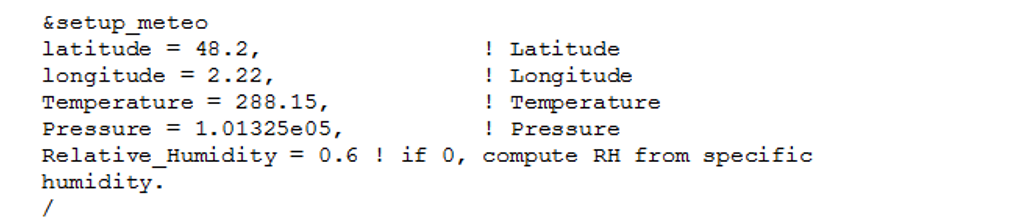
\includegraphics[angle=0,width=\textwidth]{fig/setupmeteo.png}
       \end{center}
\end{figure}

\subsection{Time}

The group setup\_time lists the initial time of the simulation (in seconds from 1$^{st}$ January), the final time (in seconds from 1$^{st}$ January) and the time step output of the simulation (in seconds). This time step corresponds to the time step when concentrations are written in the output files, but also to the time step used for splitting the resolution of gaseous chemistry, aerosol processes and emissions. Note that gaseous chemistry and aerosol processes are then solved with smaller time steps.

\begin{figure}[H]
        \begin{center}
                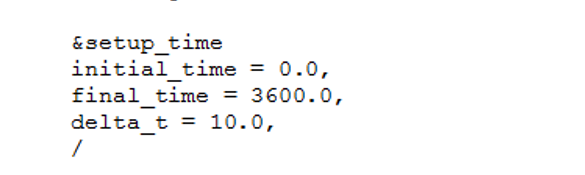
\includegraphics[angle=0,width=0.6\textwidth]{fig/setuptime.png}
       \end{center}
\end{figure}

\subsection{Initial conditions}
 
The group initial\_condition lists the initial conditions of the simulation. The number of size section is defined in the variable N\_sizebin. The variable tag\_dbd defines whether particle size bounds are either generated in the program by assuming they are equally spaced logarithmically (tag\_dbd = 0) or whether they are read (tag\_dbd = 1). If they are read, they need to be specified in the group initial\_diam\_distribution.
The variable tag\_init defines whether the particles are internally mixed (tag\_init = 0) or not (tag\_init = 1) initially. It needs to be set to 0 in the current model version.
The variable with\_init\_num defines whether number concentrations are estimated from mass concentrations and diameters of each size section (with\_init\_num = 0) or whether number concentrations are read (with\_init\_num = 1).
The variable wet\_diam\_estimation is equal to 0 if isorropia is called
initially to estimate the liquid water content of particles and the wet
diameter. If wet\_diam\_estimation is equal to 1, the initial wet diameter is
estimated from the input water concentrations (and so it is equal to the dry
diameter if water concentration is zero initially).
Finally, the names of the files containing initial gas and mass concentrations and number concentrations (if with\_init\_num = 1) are specified by the variables init\_gas\_conc\_file, init\_aero\_conc\_mass\_file and init\_num\_conc\_num\_file respectively.
The unit for gas and aerosol mass concentrations is $\mu$g~m$^{-3}$, and the unit for number concentration is \#particles~m$^{-3}$.

\begin{figure}[H]
        \begin{center}
                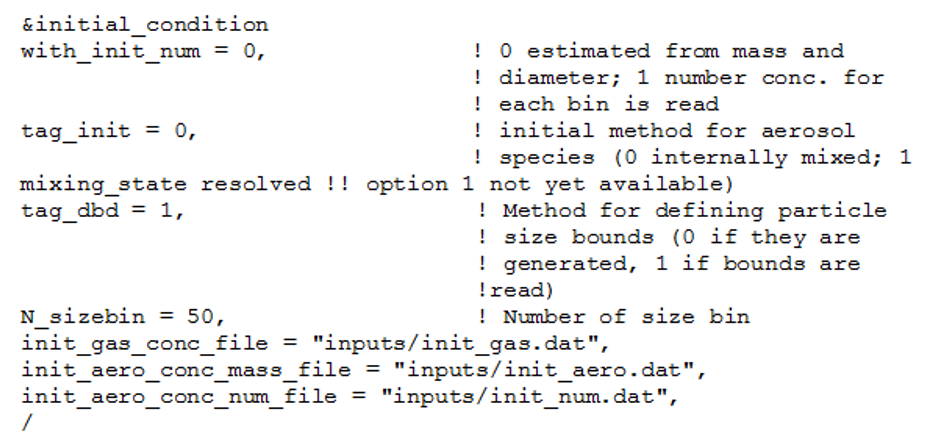
\includegraphics[angle=0,width=\textwidth]{fig/initialconditions.png}
                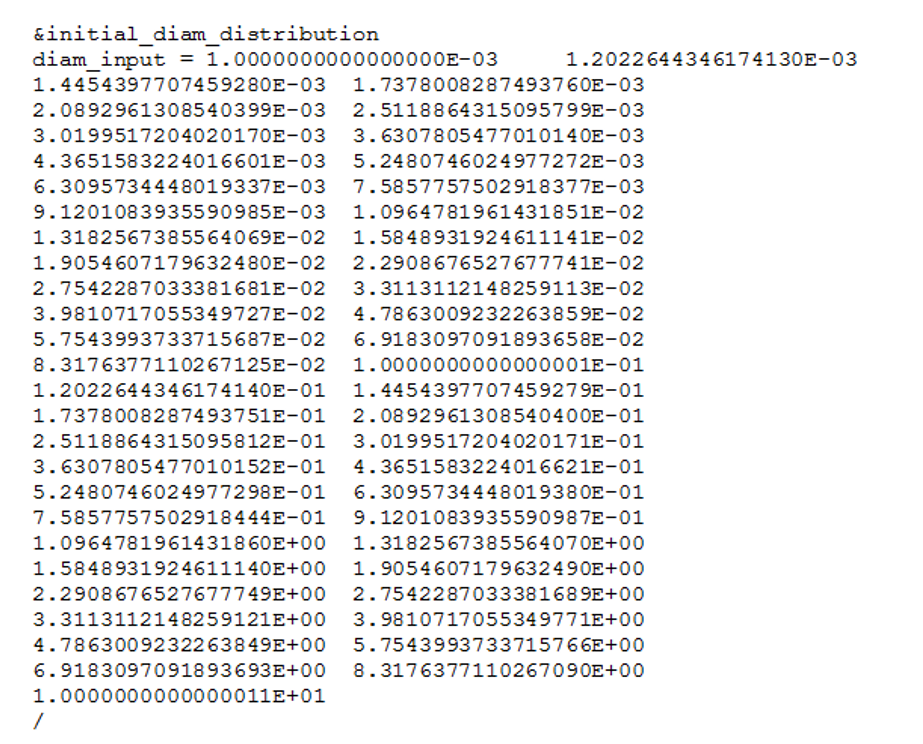
\includegraphics[angle=0,width=\textwidth]{fig/initialdiamdistribution.png}
       \end{center}
\end{figure}


\subsection{Mixing state}

The group mixing\_state defines the mixing state of particles. The variable tag\_external is set to 0 for internally-mixed particles and to 1 for mixing-state resolved particles. The variable N\_groups defines the number of group of aerosol compounds for which the composition is discretized. It is set to 1 for internal mixing, because the composition of compounds is then not discretized. In case of mixing-state resolved particles, the belonging of each compound to a group is specified in the input file detailing the aerosol compounds and their properties.
The variable N\_frac determines the number of mass fraction sections used in the discretisation of composition. 
Finally, the variable kind\_composition determines whether the fraction are discretized by the program (they are then evenly discretised, kind\_composition = 1), or whether they are read. If they are read, they need to be specified in the group fraction\_distribution.


\begin{figure}[H]
        \begin{center}
                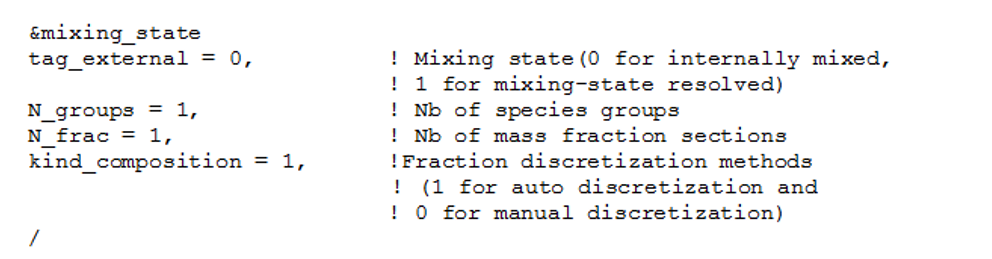
\includegraphics[angle=0,width=\textwidth]{fig/mixingstate.png}
                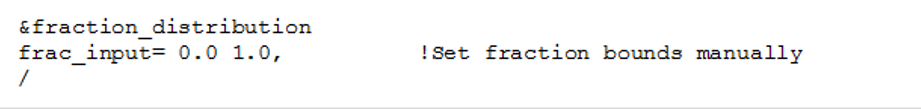
\includegraphics[angle=0,width=\textwidth]{fig/fractiondistribution.png}
       \end{center}
\end{figure}

\subsection{Gas and aerosol species}

The gas phase species are detailed in the group gas\_phase\_species, where the variable species\_list\_file contains the name of the file with the list of gas-phase species.
In this file, gas-phase species are listed together with their molar weight in g/mol. Note that the order of the species in this file should not be changed. It is set by the preprocessor of gas-phase chemical schemes.

\begin{figure}[H]
        \begin{center}
                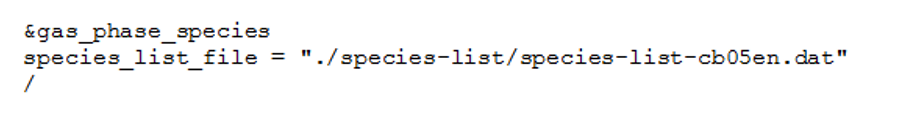
\includegraphics[angle=0,width=\textwidth]{fig/gasphase.png}
        \end{center}
\end{figure}

Aerosol species are detailed in the group aerosol\_species, where the variable aerosol\_species\_list\_file contains the name of the file with the list of aerosol species.
In this file, each aerosol species is listed on a line, together with specific properties: the group to which the species belong in case of mixing-state resolved particles, their molar weight (g/mol) and gaseous precursors, the collision factor, molecular diameter (Angstrom), surface tension (N/m), accomodation coefficient (between 0 and 1) and density in $\mu$g~$\mu$m$^3$.
The categories to which species correspond are also listed. They should not be modified and they must correspond to those set in the routine ModuleInitialisation.f90 of ssh-aerosol.

\begin{figure}[H]
        \begin{center}
                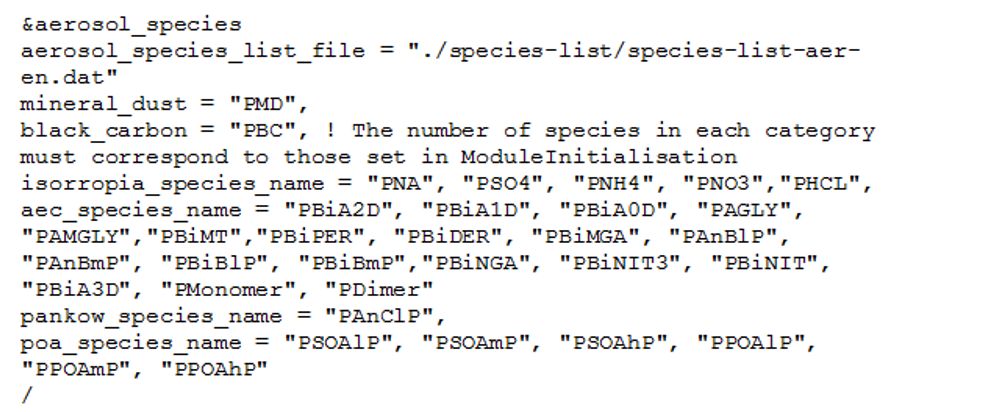
\includegraphics[angle=0,width=\textwidth]{fig/aerosolspecies.png}
        \end{center}
\end{figure}


\subsection{Emissions}

The group emissions defines options linked to emissions. The variable tag\_emis defines whether emissions are used (tag\_emis = 1) or not (tag\_emis = 0). Emissions are assumed to be internally mixed. Gas-phase emissions and/or particle-phase emissions can be specified. Number concentrations at emission may be determined from mass emissions and section diameters if the variable with\_emis\_num is set to 0. They are read from a file is the variable with\_emis\_num is set to 1. 
The name of the file containing the list of gas-phase emitted species and their emission rates should be specified using the variable emis\_gas\_file. Similarly, the name of the file containing the list of aerosol-phase emitted species and their emission rates should be specified using the variable emis\_aero\_mass\_file. Note that the unit for emission rates is $\mu$g~m$^{-3}$~s$^{-1}$. If number emissions are read, the name of the files containing emission rates should be specified using the variable emis\_aero\_num\_file. The units of number emissions should be \#particles~m$^{-3}$~s$^{-1}$.

\begin{figure}[H]
        \begin{center}
                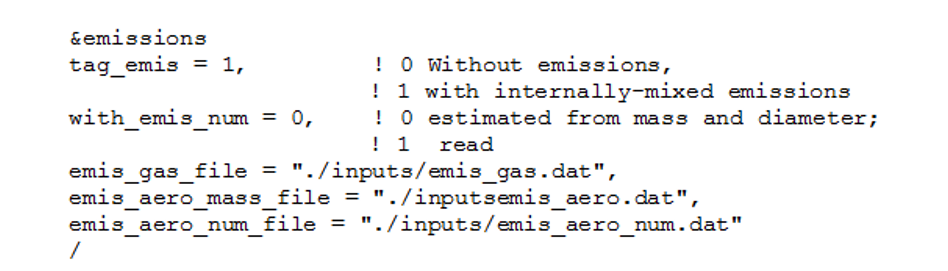
\includegraphics[angle=0,width=\textwidth]{fig/emissions.png}
        \end{center}
\end{figure}


\subsection{Numerical and physical options}

\subsubsection{Gas-phase chemistry}

The group physic\_gas\_chemistry lists options related to gas-phase chemistry. 
The variable tag\_chem defines whether gas-phase chemistry is used (tag\_chem = 1) or not (tag\_chem =0). 
Photolysis reactions may be taken into account (with\_photolysis = 1) or ignored (with\_photolysis = 0). In case photolysis reactions are taken into account, they may be attenuated by clouds. The cloud attenuation (variable attenuation) has a value below 1 in case of cloud attenuation of photolysis, and it is equal to 1 if no cloud attenuation (clear sky).
Heterogeneous reactions at the surface of particles may be taken into account (variable with\_heterogeneous = 1) or ignored (variable with\_heterogeneous = 0). An adaptive time step may be used to solve gaseous chemistry (variable with\_adaptive). It is advised to use the adaptative time step and to set the relative tolerance to decide if the time step is kept to 0.01 or 0.001. The minimum time step (in seconds) that can be used in the solver is set with the variable min\_adaptive\_time\_step.

\begin{figure}[H]
        \begin{center}
                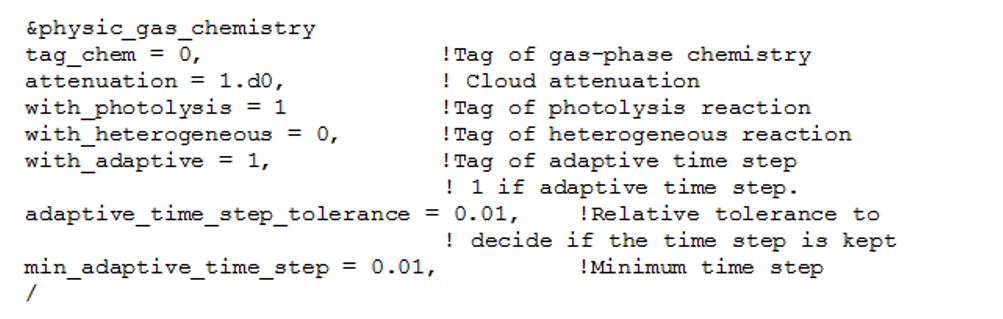
\includegraphics[angle=0,width=\textwidth]{fig/gaschemistry.png}
        \end{center}
\end{figure}

\subsubsection{Numerical issues related to aerosols}

The group physic\_particle\_numerical\_issues lists options related to numerical issues when solving aerosol dynamics. 
The variable DTAEROMIN specfies the The minimum time step (in seconds) that can be used in the solver. 
Different redistribution methods of mass and number concentrations onto the fixed diameter grids may be used (variable redistribution\_method). If only the process of condensation/evaporation is considered for aerosol dynamics, then it is possible to not apply redistribution (redistribution\_method = 0). If nucleation and/or coagulation is also considered, then a redistribution method should be chosen. It is advised to use the redistribution 10 (moving diameter) or 12 (euler coupled). The different redistributions (redistribution\_method) are euler mass (3), euler number (4), hemen (5), moving diameter (10), area-based as in SIREAM (11), euler coupled (12).
The density of particles may be computed during the simulation depending on the composition of particles if the variable with\_fixed\_density is set to 0. If it is set to 1, then the density is fixed through the simulation to the value set by the variable fixed\_density (in $\mu$g~$\mu$m$^{-3}$). Note that the variable fixed\_density needs to be set.

Numerically, the nucleation and condensation/evaporation of inorganics are always solved simultaneously, because nucleation and condensation/evaporation are competing processes. Coagulation may also be coupled to nucleation and condensation/evaporation if the variable splitting is set to 1. If splitting = 0, coagulation is splitted from nucleation and condensation/evaporation. If nucleation is taken into account, it is recommanded to set splitting to 1.

\begin{figure}[H]
        \begin{center}
                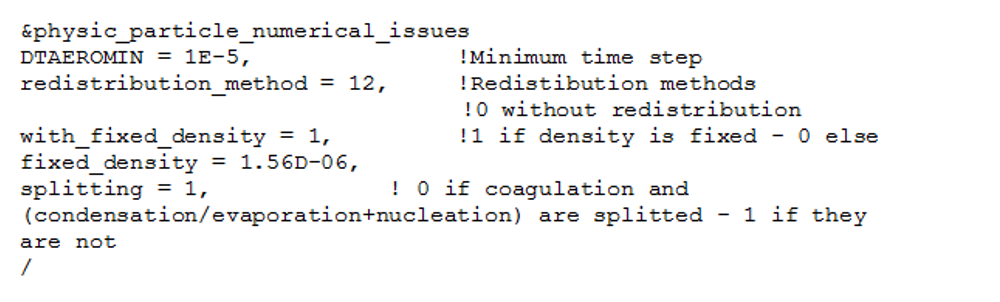
\includegraphics[angle=0,width=\textwidth]{fig/numericalissues.png}
        \end{center}
\end{figure}

\subsubsection{Coagulation}

The group physic\_coagulation lists options related to coagulation. The variable with\_coag defines whether coagulation is taken into account (with\_coag = 1) or not (with\_coag =0). 
Rapartition coefficients may be computed in the simulation (i\_compute\_repart = 1) or read from a netcdf file (i\_compute\_repart = 0). If they are read from a file, its name should be specified (Coefficient\_file). If they are computed, the number of Monte Carlo points used to compute them should be specified (Nmc). This number should be large enough and its value depends on the section discretization used.


\begin{figure}[H]
        \begin{center}
                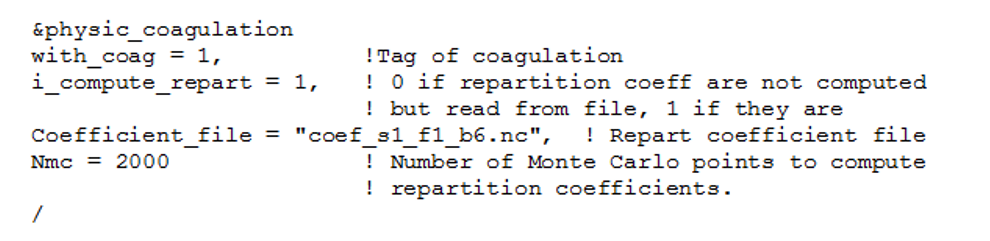
\includegraphics[angle=0,width=\textwidth]{fig/coagulation.png}
        \end{center}
\end{figure}
          
\subsubsection{Condensation/evaporation}

The group physic\_condensation lists options related to condensation/evaporation. The variable with\_cond defines whether condensation/evaporation is taken into account (with\_cond = 1) or not (with\_cond =0). Kelvin effect may be taken into account (with\_kelvin\_effect = 1), as recommanded if ultrafine particles are simulated, or ignored (with\_kelvin\_effect = 0).
For the condensation/evaporation of inorganic compounds, Cut\_dim corresponds to the diameter under which thermodynamic equilibrium is assumed. Set it to 0 to compute dynamically condensation/evaporation for all particles, and set it to a value larger than larger diameter to assume thermodynamic equilibrium.
For the condensation/evaporation of organic compounds, ISOAPDYN determines whether thermodynamic equilibrium is assumed for all particles (ISOAPDYN = 0) or whether condensation/evaporation is computed dynamically (ISOAPDYN = 1). Even if it is computed dynamically, thermodynamic equilibrium may be used for the condensation/evaporation of small particles by setting a characteristic time under which equilibrium is assumed for organics (e.g. tequilibrium = 0.1 seconds). For numerical reasons, tequilibrium may not be set to 0, but condensation/evaporation of all particles is solved dynamically if (ISOAPDYN = 1) and tequilibrium is set to a small value (e.g. 1.d-15). In the current version of the code, the diffusion coefficient dorg in the organic phase is assumed constant. Typical values would be 1.d-12 for non viscous particles and 1.d-23 for very viscous particles. 
The variable coupled\_phases should be set to 1 if the resolution os the aqueous and organic phases is coupled and to 0 if they are solved independently. The interactions between compounds in the particles may be assumed to be ideal (activity\_model = 1), or activity coefficients may be computed with unifac (interactions between organics only, activity\_model = 2) or with aiomfac (activity\_model = 3).

\begin{figure}[H]
        \begin{center}
                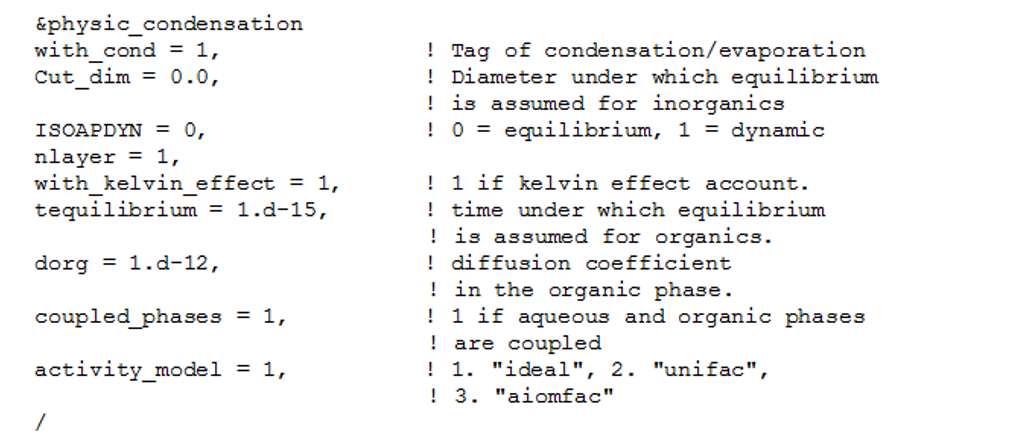
\includegraphics[angle=0,width=\textwidth]{fig/condensation.png}
        \end{center}
\end{figure}
          
\subsubsection{Nucleation}


The group physic\_nucleation lists options related to nucleation. The variable with\_nucl defines whether nucleation is taken into account (with\_nucl = 1) or not (with\_nucl =0). If nucleation is taken into account, then the lower diameter bound should be about 1 nm. Three nucleation models are implemented.
\begin{itemize}
\item binary: water and sulfate with the parameterisation of \cite{vehk} (nucl\_model = 0)
\item ternary: water, sulfate and ammonium with the parameterisation of \cite{napari} (nucl\_model = 1) or with the parameterisation of \cite{merikantoa, merikantob} (nucl\_model = 2).
To avoid artificially large nucleation rates in the parameterisation of \cite{napari}, a maximum nucleation rate of 1.d6 \#particles~cm$^{-3}$ is set.
\end{itemize}


\begin{figure}[H]
        \begin{center}
                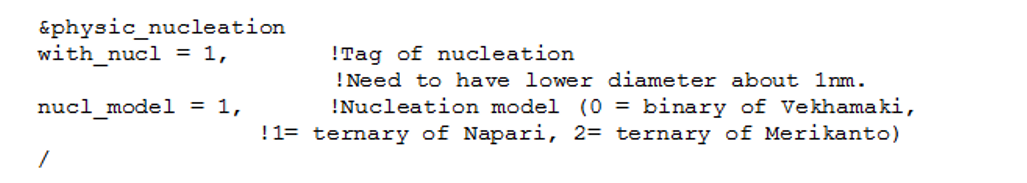
\includegraphics[angle=0,width=\textwidth]{fig/nucleation.png}
        \end{center}
\end{figure}
          

\subsubsection{Organics}

Concerning organic reactions in the particles, oligomerization of pinonaldehyde may be considered (with\_oligomerization = 1) or not.

\begin{figure}[H]
        \begin{center}
                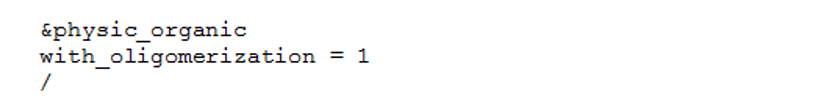
\includegraphics[angle=0,width=\textwidth]{fig/organic.png}
        \end{center}
\end{figure}
 

\subsection{Output}

The output directory may be specified, as well as the format of the files (text if output\_type = 1, and binary if output\_type = 2).
 
\begin{figure}[H]
        \begin{center}
                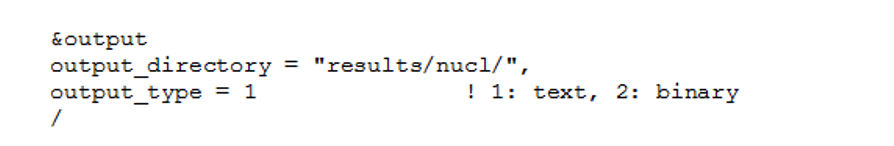
\includegraphics[angle=0,width=\textwidth]{fig/output.png}
        \end{center}
\end{figure}
               
\section{Test cases}
\addcontentsline{toc}{section}{Test cases}

This section presents a few test-cases to demonstrate how the model works.

During the practical session, we will work in the directory
\cmd{ssh-aerosol}. 
To compile the program, please type {\it{compile}}. Before compiling, you may
clean previous compilation by typing {\it{clean}}.

The main options of the simulations are detailed in the namelist files (for
example {\it{INIT/namefile\_coag.ssh}}), which are in the folder {\it{INIT}}, and
initial conditions (meteorological, gas and aerosol concentrations) are
required.
The simulation can be run by typing {\it{ssh-aerosol INIT/namefile\_coag.ssh}}.

The list of species and parameters are detailed in the files {\it{species-list/species-list-aer-en.dat}} and {\it{species-list/species-list-cb05en}}. The name and location of the files can be modified in the configuration file {\it{namelist*.ssh}}.

Different processes can be considered (set the flag to 1) or ignored (set the flag to 0): emissions (flag {\it{tag\_emis}}),
gaseous chemistry (flag {\it{tag\_chem}}),
coagulation (flag {\it{with\_coag}}),
condensation (flag {\it{with\_cond}}),
nucleation (flag {\it{with\_nucl}}).
Internal mixing (flag {\it{tag\_external}} set to 0) or mixing-state resolved particles (flag {\it{tag\_external}} set to 1) can be considered. 

\subsection{Dynamic of coagulation and condensation}

In the literature, to test the overall behavior of PM models, the following 
basic tests of
condensation and coagulation of sulfate are often considered \cite{seigneur1986simulation,zhang1999simulation,binkowski2003models}. A tri-modal PM distribution is considered initially,
with particles being made exclusively of sulfate. The parameters of the initial distribution
considered here are those of hazy conditions for the condensation test with a sulfuric
acid production rate of 9.9 $\mu$g m$^{-3}$, and those of urban conditions for the coagulation test \cite{seigneur1986simulation,zhang1999simulation} , because these two tests represent the two most
stringent conditions for coagulation and condensation. Temperature is taken as 283.15 K.
Simulations are conducted for 12 hours.
The reference solutions for the coagulation and condensation tests are those of \cite{zhang1999simulation} obtained with another models.


\subsubsection{Coagulation}
\label{coag-test}

The configuration file for this test is {\it{namelist\_coag.ssh}}.
In the coagulation test case, only coagulation is considered by setting the variable of {\it{with\_coag}} of the file {\it{namelist\_coag.ssh}} to 1.

The partition coefficients may be precomputed in a C++ routine. Here, the
coefficients are directly computed by ssh-aerosol (option {\it{i\_compute\_repart}}), using a
Monte-Carlo method (Nmc represents the Monte Carlo number). The larger Nmc is,
the more accurate the coefficients are, but the more CPU time it takes to
compute them.
Run the simulation by typing {\it{ssh-aerosol INIT/namelist\_coag.ssh}}.
You can compare the number and volume distribution of particles at the initial
time and after 12~h by going to the repertory {\it{graph}} and by running the
python script {\it{dN\_Vdlogd\_coag.py}}.
ssh-aerosol does very well in representing the growth of particles by
coagulation, as shown in Fig~\ref{fig-coag}.

\begin{figure}[H]
        \begin{center}
                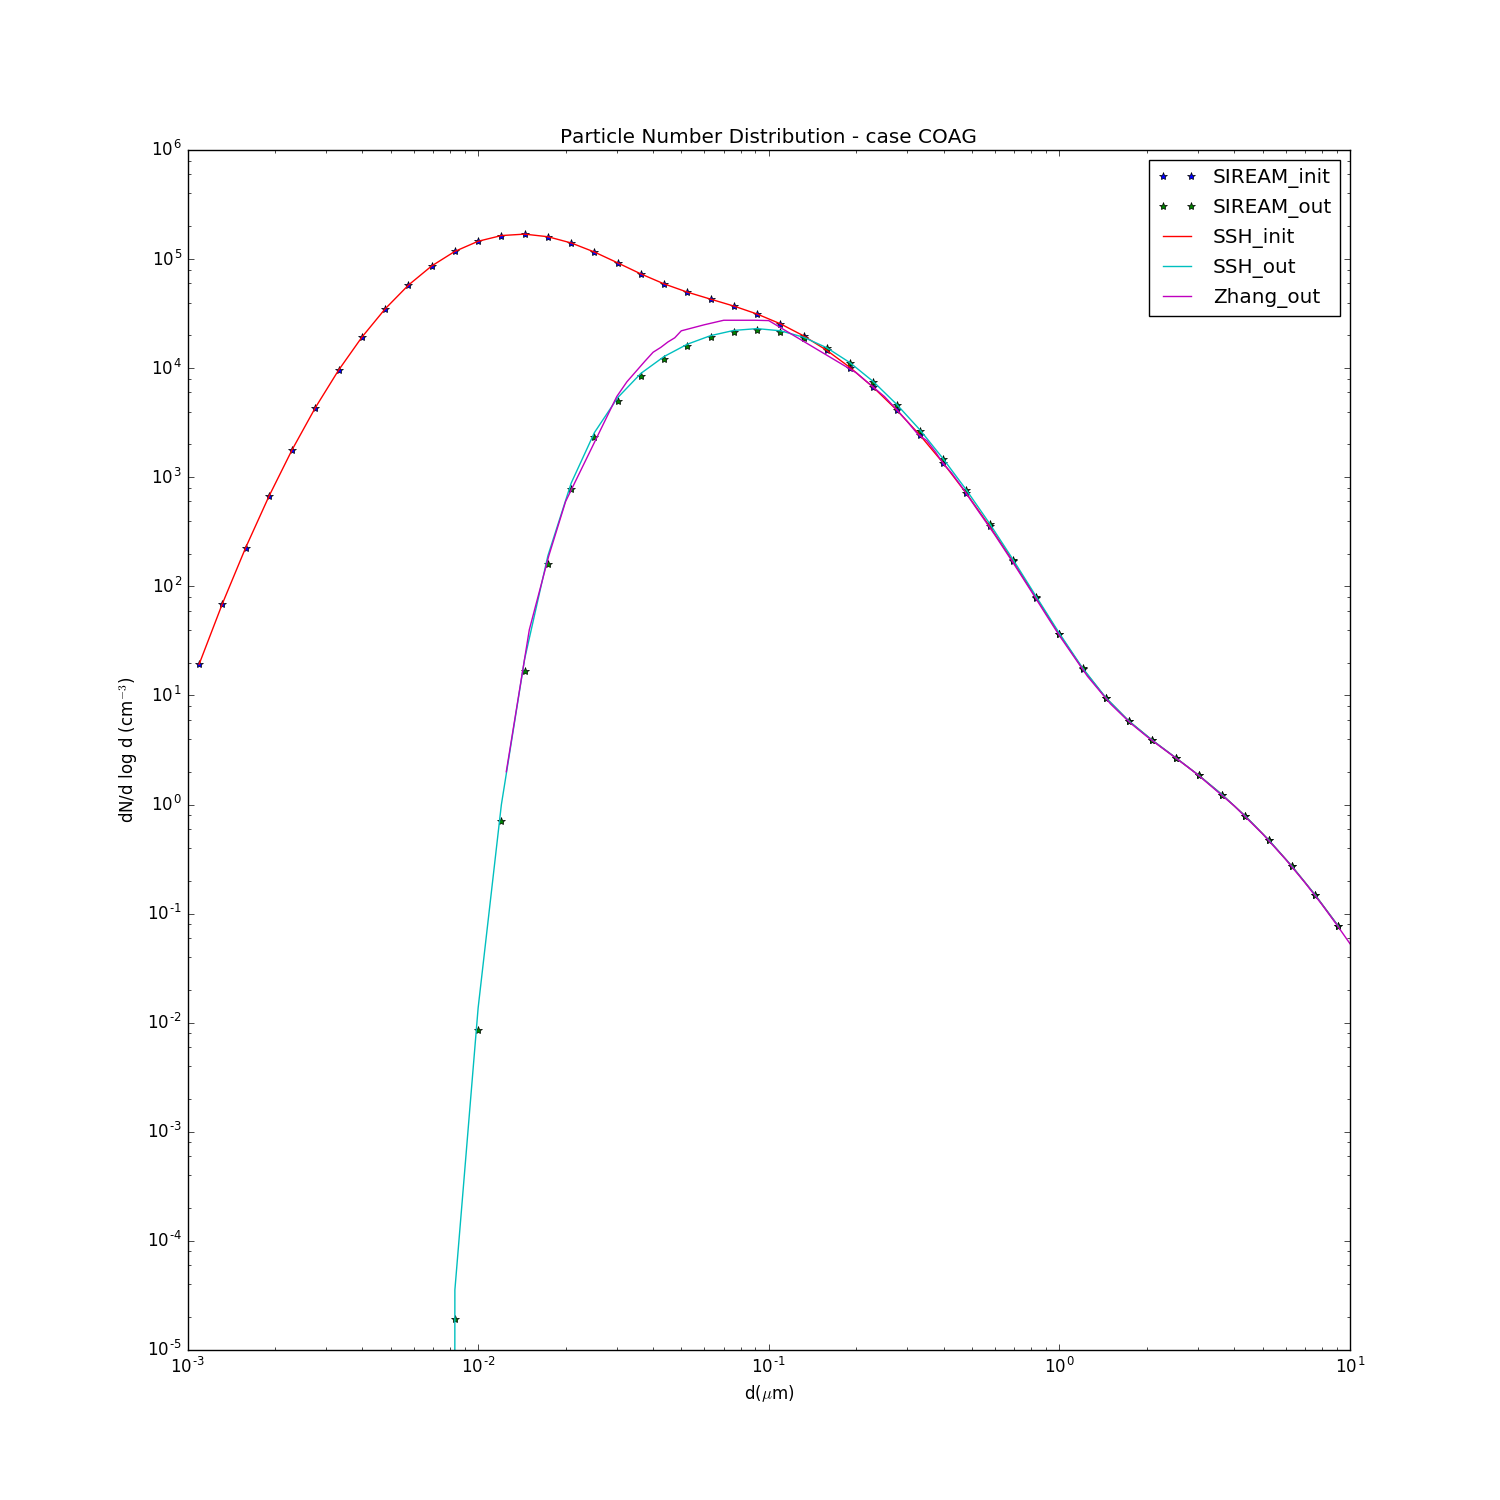
\includegraphics[angle=0,width=0.45\textwidth]{../graph/figure_ref/dNdlogd_COAG.png}
                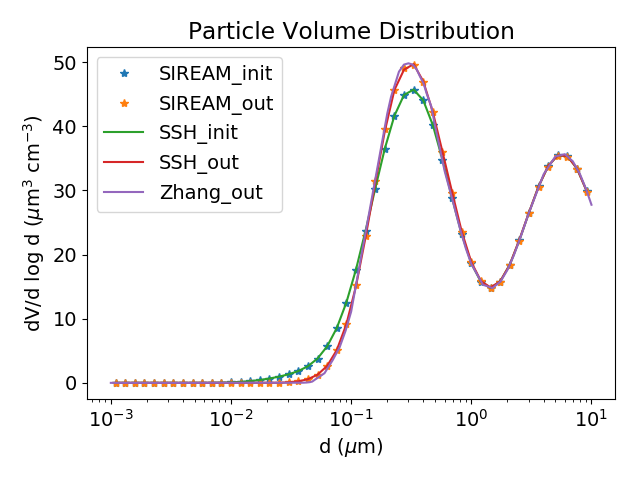
\includegraphics[angle=0,width=0.45\textwidth]{../graph/figure_ref/dVdlogd_COAG.png}
        \end{center}
\caption{Coagulation test case. Number (left panel) and volume (right panel) concentrations.}
\label{fig-coag}
\end{figure}
        
\subsubsection{Condensation of sulfate}
\label{cond-sulf}

The condensation test with hazy conditions is very stringent, because the high condensation
rate lead to a narrow Aitken mode.
The configuration file for this test is {\it{namelist\_cond.ssh}}.
Only condensation/evaporation is considered by setting the variable {\it{with\_cond}} of the file {\it{namelist.ssh}} to 1.

Run the simulation by typing {\it{ssh-aerosol INIT/namelist\_cond.ssh}}.
You can compare the number and volume distribution of particles at the initial
time and after 12~h by going to the repertory {\it{graph}} and by running the
python script {\it{dN\_Vdlogd\_cond.py}}.
ssh-aerosol does very well in representing
the Aitken mode as well as the growth of the accumulation mode if no
redistribution is used ({\it{redistribution\_method}} = 0 in
{\it{namelist\_cond.ssh}}), as shown in Fig~\ref{fig-cond-noredist}. 

Redistributing the mass and number concentrations
amongst bins lead to numerical diffusion, as can be seen by using the
redistribution methods 10 (moving diameter), 11 (area-based (siream)) or 12
(euler-coupled) (see Fig~\ref{fig-cond-redist}).
You can change the redistribution by changing the flag {\it{redistribution\_method}}.

In order to use a growth law, which is as close as possible to the original growth law
used in \cite{zhang1999simulation} , the accommodation coefficient is set to 1. It is however interesting
to notice the sensitivity of results to the choice of the accommodation coefficient. 
The growth of the Aitken mode is strongly reduced by decreasing the
accommodation coefficient from 1 to 0.1.
You can change the accomodation coefficient in the file {\it{species-list/species-list-aer-en.dat}}.

\begin{figure}[H]
        \begin{center}
                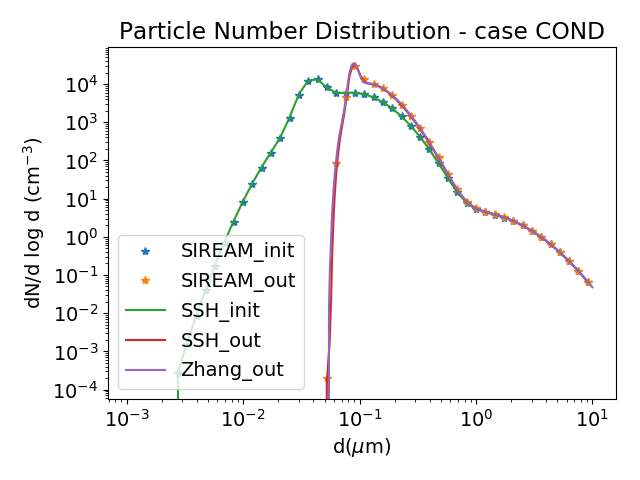
\includegraphics[angle=0,width=0.45\textwidth]{../graph/figure_ref/dNdlogd_COND_no_redist.png}
                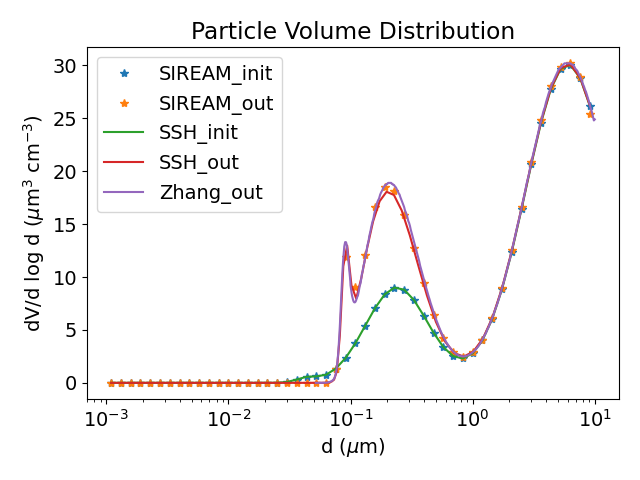
\includegraphics[angle=0,width=0.45\textwidth]{../graph/figure_ref/dVdlogd_COND_no_redist.png}
        \end{center}
\caption{Condensation test case without redistribution. Number (left panel) and volume (right panel) concentrations.}
\label{fig-cond-noredist}
\end{figure}
       
\begin{figure}[H]
        \begin{center}
                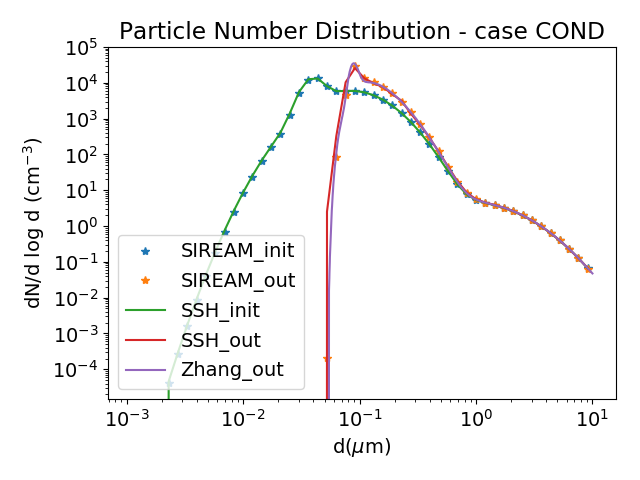
\includegraphics[angle=0,width=0.45\textwidth]{../graph/figure_ref/dNdlogd_COND_r12.png}
                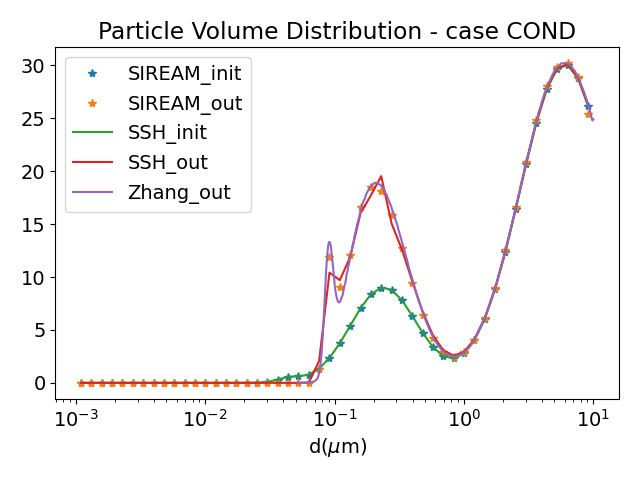
\includegraphics[angle=0,width=0.45\textwidth]{../graph/figure_ref/dVdlogd_COND_r12.png}
        \end{center}
\caption{Condensation test case with Euler-coupled redistribution. Number (left panel) and volume (right panel) concentrations.}
\label{fig-cond-redist}
\end{figure}
       
\subsubsection{Condensation of low-volatility organics}

Extremely-low volatility organic compounds (ELVOCs) are formed from the ozonolysis of monoterpenes \cite{chrit2017modelling} .
Similarly to sulfate, these compounds have a very low saturation vapor pressure and they therefore should condense with a kinetic similar to sulfate if they had the same density.
The test case on the sulfate condensation is redone with the ELVOC Monomer, by artificially setting its density to that of sulfate.
The configuration file for this test is {\it{namelist\_cond\_monomer.ssh}}.
The monomer density is modified in the file {\it{species-list-monomer/species-list-aer-en.dat}}.
In the input files for initial conditions {\it{init\_gas.dat}} and {\it{init\_aero.dat}} of the directory {\it{inputs/inputs-cond-monomer/}}, initial concentrations are assigned to monomer rather than sulfate. You can plot the number and volume distribution by using the python script {\it{graph/dN\_Vdlogd\_cond\_monomer.py}}. 
The distributions are similar to those of the sulfate case.

\subsubsection{Condensation/evaporation of inorganics}
For inorganic compounds, differences between the particle compositions computed using equilibrium and dynamical sectional models have been stressed by numerous authors such as \cite{sartelet2006development} . This test case simulates the test case of the highly polluted day of 25 June 2001 of \cite{sartelet2006development} .
Measurements of PM and gaseous species made in Tokyo (Japan) are taken as initial conditions. Because the data were averaged continuously during 24 hours under varying meteorological conditions, this study can not assess the importance of the equilibrium approach compared to the dynamical approach. The model results obtained after thermodynamic equilibrium is reached are then compared.

The configuration file for this test is {\it{namelist\_cond-evap-inorg.ssh}} for the case where condensation/evaporation is dynamic. 
Only condensation/evaporation is considered by setting the variable of {\it{namelist\_cond-evap-inorg.ssh}} {\it{with\_cond}} to 1.
The variable {\it{Cut\_dim}} corresponds to the diameter until which thermodynamic is assumed. It is set to 0 to solve the condensation/evaporation with a dynamic approach. 

To compare this simulation to a simulation where thermodynamic equilibrium is assumed for condensation/evaporation, please set  {\it{Cut\_dim}} to 40 (the maximum diameter of the particles considered here). 
This is done in the configuration file {\it{namelist\_cond-evap-inorg-eq.ssh}}.

To assess the differences between these simulations, you can compare the time evolution of NH$_3$ and HNO$_3$, 
by running the python script {\it{graph/gas\_cond-evap.py}}. As shown in
Fig~\ref{fig-cond-evap}, the gas-phase concentrations quickly reach
thermodynamic equilibrium.


\begin{figure}[H]
        \begin{center}
                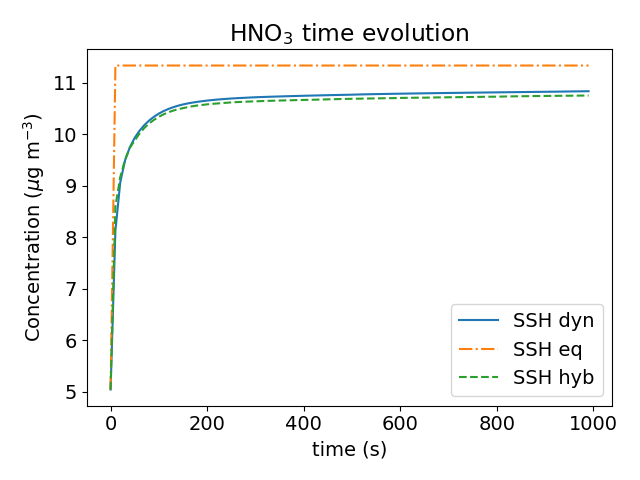
\includegraphics[angle=0,width=0.45\textwidth]{../graph/figure_ref/HNO3_COND-EVAP_time.png}
                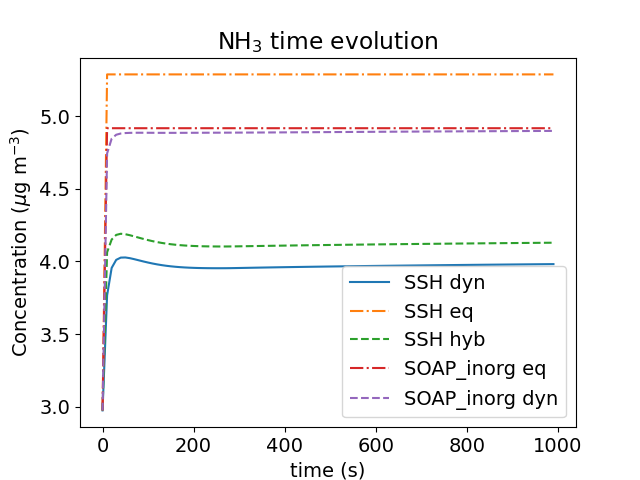
\includegraphics[angle=0,width=0.45\textwidth]{../graph/figure_ref/NH3_COND-EVAP_time.png}
        \end{center}
\caption{Condensation/�vaporation of inorganic test case. Time evolution of
  HNO$_3$ concentrations (left panel) and NH$_3$ concentrations (right panel).}
\label{fig-cond-evap}
\end{figure}
       

\subsubsection{Kelvin effect}

To illustrate the importance of the Kelvin effect for the growth of ultrafine
particles, the test case of \cite{devilliers2013new} concerning the growth of
ultrafine particles emitted from the exhaust of a diesel engine was simulated.
As in \cite{devilliers2013new}, a typical diesel engine emission initial
distribution from \cite{kittelson2006road} is used here to
study the gas/particle conversion of nonadecane (C19H40). It has a
reference saturation vapor pressure of 6.1~10$^{-4}$ Pa at T = 298 K, which is
very close to that of the model compound POAmP.
Particles are assumed here to consist solely of POAmP.
To show the importance of the Kelvin effect, two simulations are conducted:
with and without the Kelvin effect.

The configuration files for this test are {\it{namelist\_kelvin.ssh}} for the
case where the Kelvin effect is modelled, and {\it{namelist\_kelvin\_nokelv.ssh}} for the
case where it is not.
The variable {\it{ISOAPDYN}} is set to 1 to indicate that the
condensation/evaporation of organics is modelled dynamically. The variable
{\it{with\_kelvin\_effect}} is also set to 1 to take into account the Kelvin
effect in the configuration file {\it{namelist\_kelvin.ssh}} and to 0 in the configuration file {\it{namelist\_kelvin\_nokelv.ssh}}.

To compare the number and volume size distribution simulated with and without
Kelvin effect, you can run the python script {\it{graph/dN\_Vdlogd\_kelvin.py}}.

The results in Fig~\ref{fig-kelvin} show clearly that the Kelvin effect must be taken into account when
the evolution of small particles is simulated: particles are much less affected by
condensation/evaporation when it is not included in the model. The ultrafine particles of the initial distribution have been transferred to the gas phase while the coarse ones have grown to a greater size range.



\begin{figure}[H]
        \begin{center}
                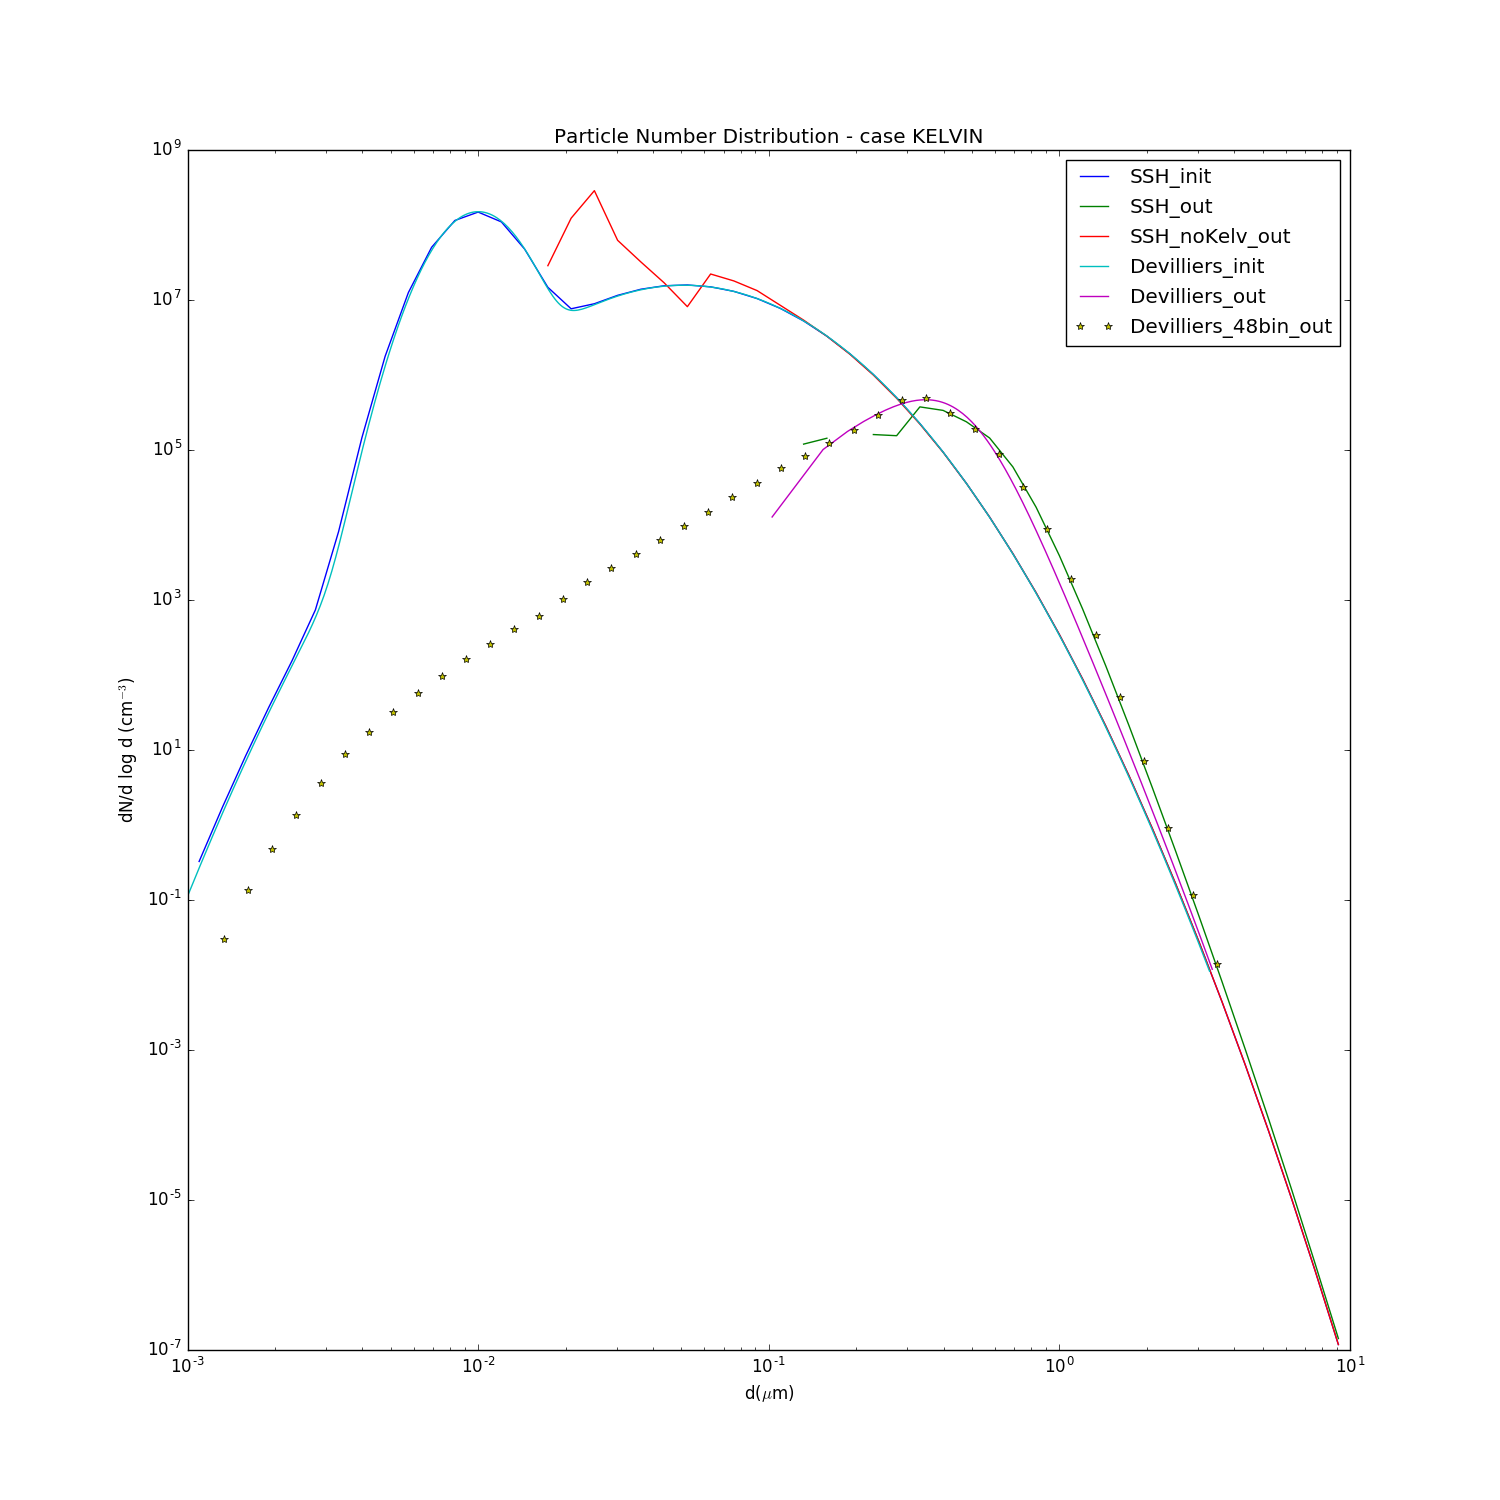
\includegraphics[angle=0,width=0.45\textwidth]{../graph/figure_ref/dNdlogd_KELVIN.png}
                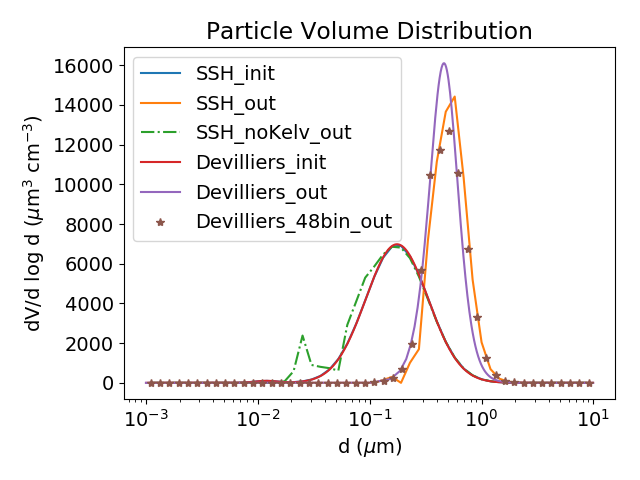
\includegraphics[angle=0,width=0.45\textwidth]{../graph/figure_ref/dVdlogd_KELVIN.png}
        \end{center}
\caption{Kelvin test case. Number (left panel) and volume (right panel) concentrations.}
\label{fig-kelvin}
\end{figure}
       
\subsubsection{Nucleation}

To assess the ability of ssh-aerosol to deal with simultaneous strong coagulation and condensation/nucleation, the nucleation test case presented in \cite{sartelet2006development} is simulated. The initial distribution is the same as in the condensation of sulfuric acid test case of section~\ref{cond-sulf}. It corresponds to the hazy conditions of \cite{seigneur1986simulation}. The sulfuric
acid production rate is 0.825~$\mu$g~m$^{-3}$~h$^{-1}$,
the temperature is 288.15 K and the relative humidity is 60\%. The particles are initially assumed to be made of 70\% sulfate and 30\% ammonium. The initial gas phase ammonia concentration is taken to be 8~$\mu$g~m$^{-3}$. The concentrations of gas phase ammonia and particulate-phase ammonium evolve with time due to both nucleation and condensation/evaporation
The ternary nucleation of \cite{napari} is used, but to avoid artificially large nucleation rates in the parameterisation of \cite{napari}, a maximum nucleation rate of 1.d6 \#particles~cm$^{-3}$ is set.
The simulation is run for 1~h with output every 60~s.

Two simulations are run: one where the processes (coagulation,
condensation/evaporation and nucleation) are solved simultaneously
(configuration file {\it{namelist\_nucl.ssh}}), and one where the numerical
resolution of coagulation is splitted from condensation/evaporation and
nucleation (configuration file {\it{namelist\_nucl\_split.ssh}}). 


To compare the number and volume size distribution simulated with the two numerical algorithms, you can run the python script {\it{graph/dN\_Vdlogd\_nucl.py}}.

The two numerical algorithms give similar number concentrations, except for
particles of diameter below 2~nm, which are over-estimated when coagulation is
splitted from condensation/evaporation. For such small particles, the combined
effects of coagulation, nucleation and condensation is important, as shown in Fig~\ref{fig-nucl}.

The nucleated particles clearly grow to larger particles with time, as can be seen both in Fig~\ref{fig-nucl2} and by running the python script {\it{graph/banana.py}}.


\begin{figure}[H]
        \begin{center}
                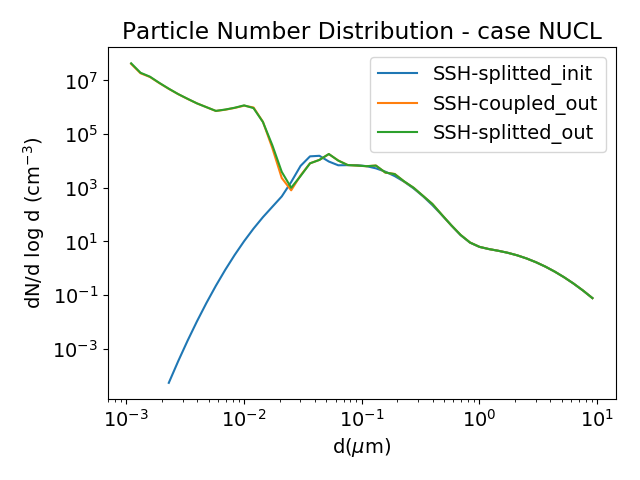
\includegraphics[angle=0,width=0.45\textwidth]{../graph/figure_ref/dNdlogd_nucl.png}
                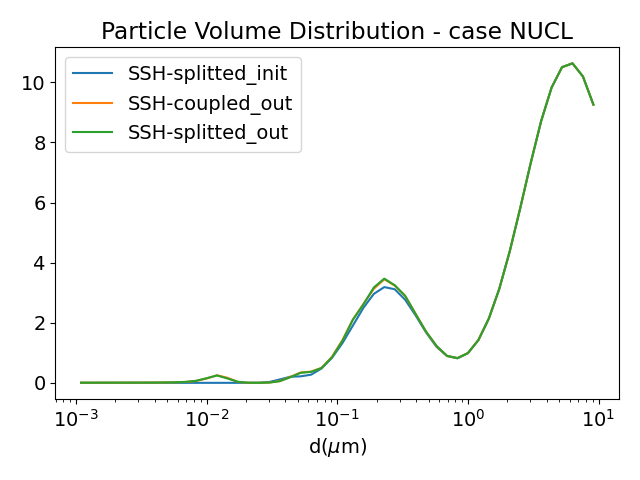
\includegraphics[angle=0,width=0.45\textwidth]{../graph/figure_ref/dVdlogd_nucl.png}
        \end{center}
\caption{Nucleation test case. Number (left panel) and volume (right panel) concentrations.}
\label{fig-nucl}
\end{figure}
       

\begin{figure}[H]
        \begin{center}
                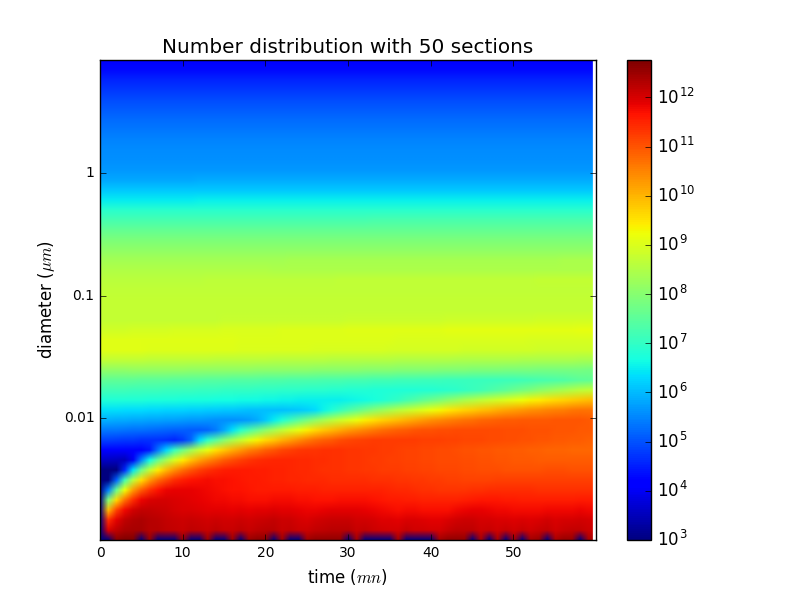
\includegraphics[angle=0,width=0.45\textwidth]{../graph/figure_ref/fig_banana.png}
        \end{center}
\caption{Nucleation test case. Time evolution of the number concentrations.}
\label{fig-nucl2}
\end{figure}
       

\subsection{Modelling of aerosol formation}

After emission into the atmosphere, the oxidation of volatile organic compounds (VOCs) leads to less volatile compounds than the precursors. 
These compounds condense more easily onto particles than their precursors and they contribute to the increase of particle mass.

\cite{platt2013secondary} performed ageing experiments on emissions from an Euro 5 gasoline car. They monitored the total hydrocarbon mass (THC) as well as organic aerosol (OA) concentrations. 
The test case presented here corresponds to the simulation performed in \cite{sartelet2018emission}.

In our model, THC is assumed to be the sum of VOC and I/S VOCs (intermediate and semi-volatile VOCs). THC is initialized as measured in the experiments of \cite{platt2013secondary} before lights-on (1.4 ppmv + 0.9 ppmv of propene). IVOCs are estimated from VOC emissions using the ratio 0.17 estimated by \cite{zhao2016intermediate}, and NOx concentrations are initialized such as having a VOC/NOx ratio equal to 5.6 as in \cite{platt2013secondary} . 
The speciation of VOCs to model species was done following \cite{theloke2007compilation}.

The configuration file for this test is {\it{namelist\_platt.ssh}}.

Not only condensation/evaporation is considered by setting the variable of {\it{namelist\_platt.ssh}} {\it{with\_cond}} to 1, but also gaseous chemistry ( {\it{tag\_chem}}=1). Photolysis rates are predefined in this version of ssh, and a more accurate representation of those (similar to what is used in 3D) will be implemented soon.

After running the model for 5~h, the evolution of the aerosol concentrations with time may be displayed by running the script {\it{plot\_platt\_particles.py}}.
As in the experiment after correction for wall loss, the concentrations of
particles is about 200~$\mu g$~$m^{-3}$. More than half of the mass origins
from the condensation/evaporation of aged I/S VOCs, as shown in Fig~\ref{fig-platt}.
The inorganic concentrations stay low (5~$\mu g$~$m^{-3}$ of sulfate was introduced initially as a seed and does not vary during the simulation; and nitrate stays below 9~$\mu g$~$m^{-3}$).
% If NH3 is introduced, large amounts of inorganic concentrations are formed
% Barbara.

\begin{figure}[H]
        \begin{center}
                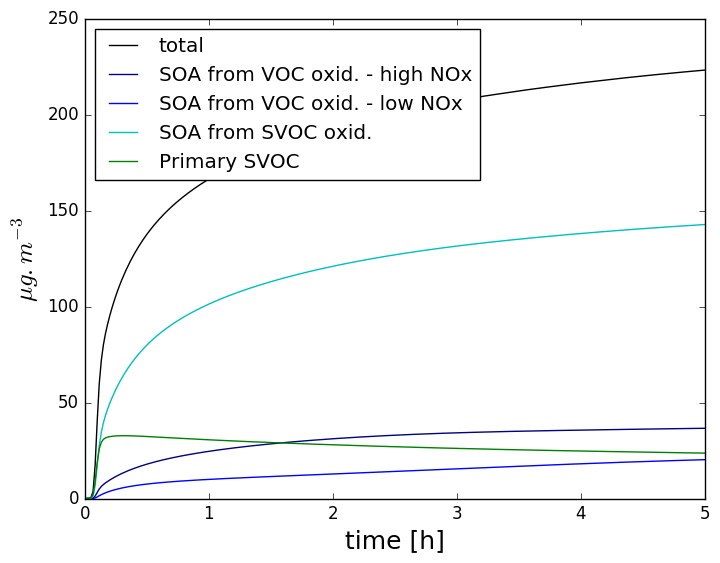
\includegraphics[angle=0,width=0.45\textwidth]{../graph/figure_ref/platt-particles.png}
        \end{center}
\caption{Platt test case. Time evolution of organic concentrations.}
\label{fig-platt}
\end{figure}
       
\subsection{Mixing state}
The previous test cases relied on the internal mixing assumption (one aerosol
composition per aerosol size section).
The internal mixing assumption relies on the assumption that particles from different sources
mix instantaneously when they are present in the same air mass. Although this assumption may
be realistic far from emission sources, it may be difficult to justify close to emission sources,
where emitted particles can have compositions that are very different from background particles
and from particles emitted from different sources.
All aerosol dynamic processes may affect the mixing state of particles.

\subsubsection{Coagulation}

To illustrate how coagulation affects the mixing state of particles, the
coagulation test case (see section~\ref{coag-test}) is revisited by assuming
that the initial aerosol distribution is made of two low-volatility compounds
of same density (sulfate and another low-volatility compound).
The configuration file for this test is {\it{namelist\_coag\_ext.ssh}}.
In this coagulation test case, the composition is discretized using 4 sections
by setting the variable {\it{N\_frac}} to 4. The bound values of the fraction
sections are specified using the variable {\it{frac\_input}}.

Run the simulation by typing {\it{ssh-aerosol INIT/namelist\_coag\_ext.ssh}}.
By summing the mass and number of particles of all size fraction sections, the
size number and volume distribution are identical to those obtained with the
internal mixing assumptions. This can be checked by going to the repertory
{\it{graph}} and by running the python script {\it{dN\_Vdlogd\_coag\_ext.py}}
(see Fig~\ref{fig-coag-ext}).
The evolution of the mixing-state of particles after 12 h of coagulation may
be seen by comparing the two panels in Fig~\ref{fig-coag-extb}, which shows
the number concentrations as a function of the size and fraction of one
sulfate, which is one of the
two compounds of the particles.

\begin{figure}[H]
        \begin{center}
                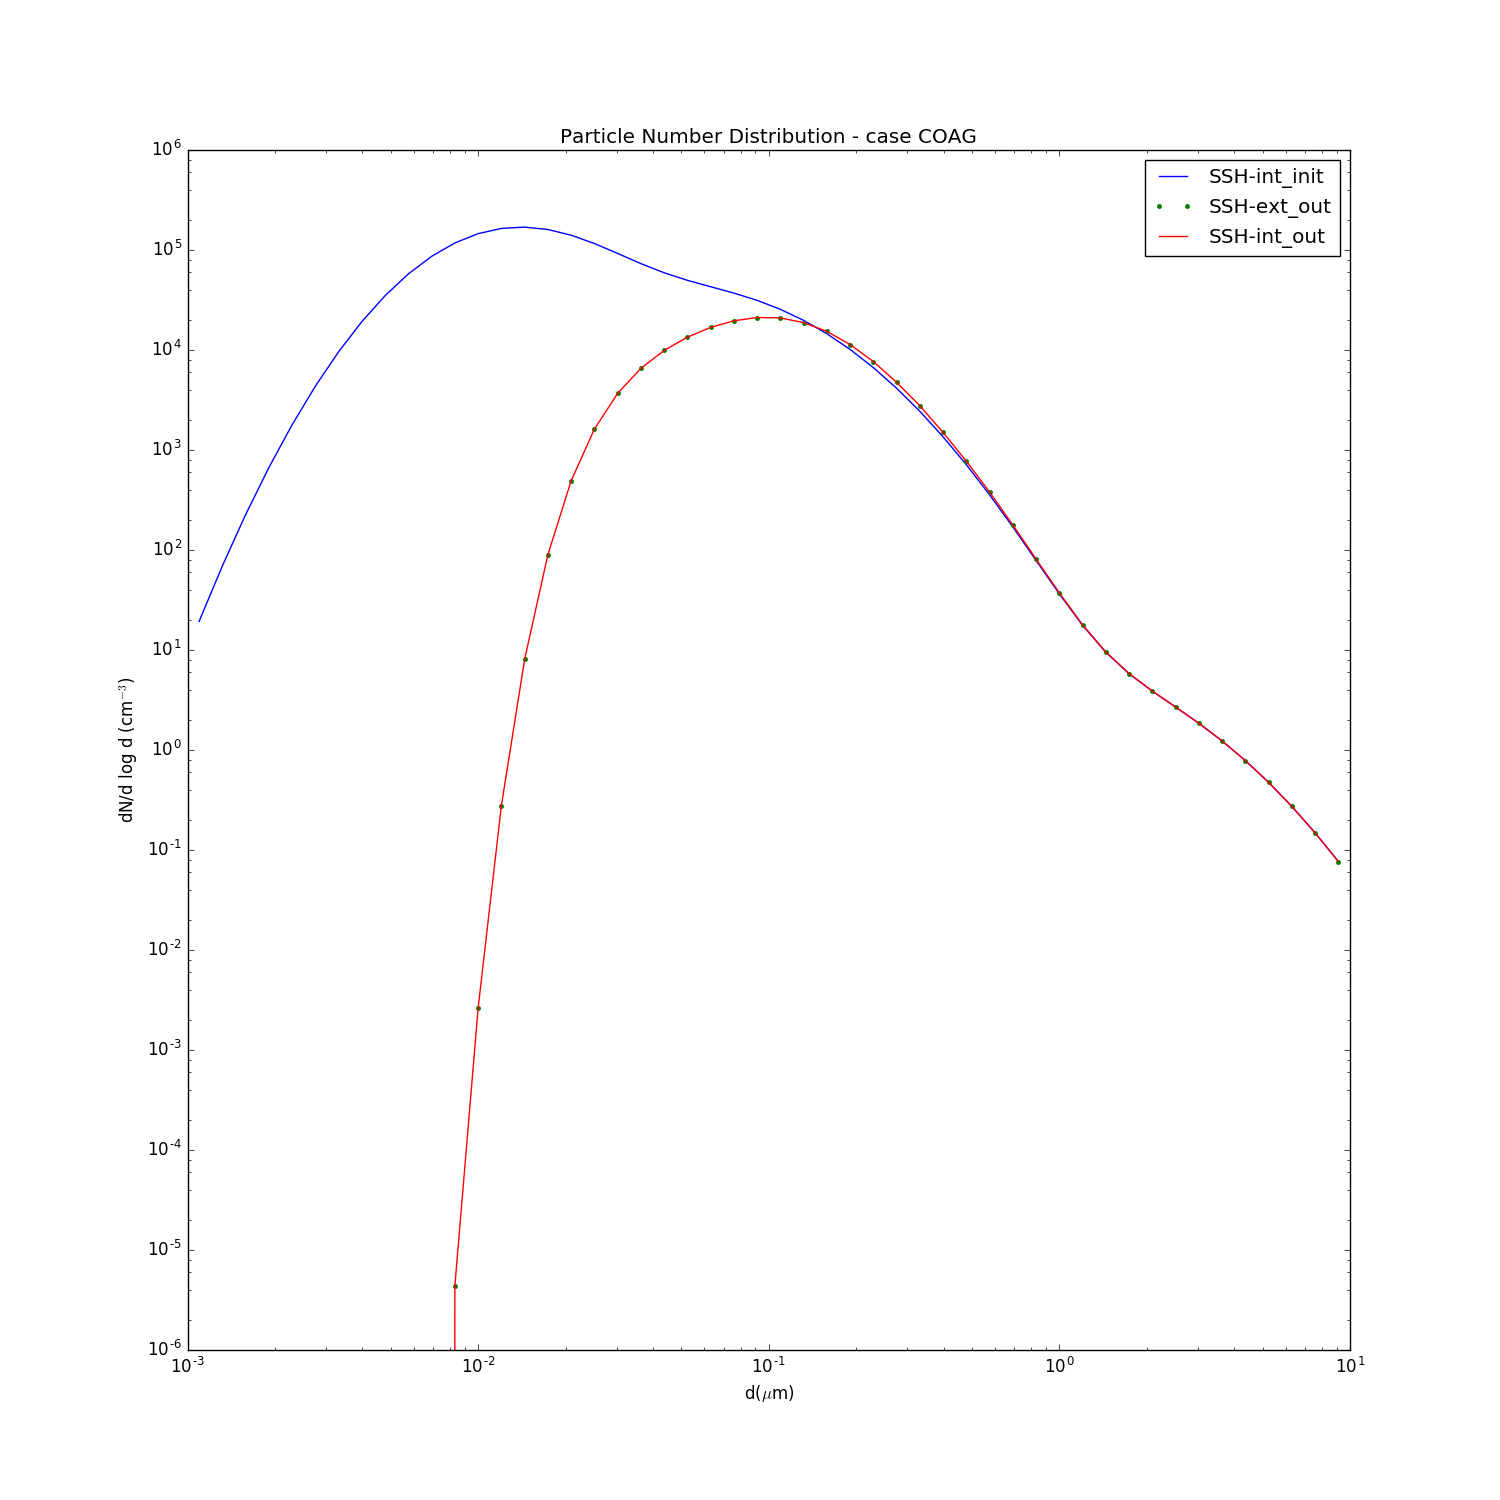
\includegraphics[angle=0,width=0.45\textwidth]{../graph/figure_ref/dNdlogd_COAG_EXT.png}
                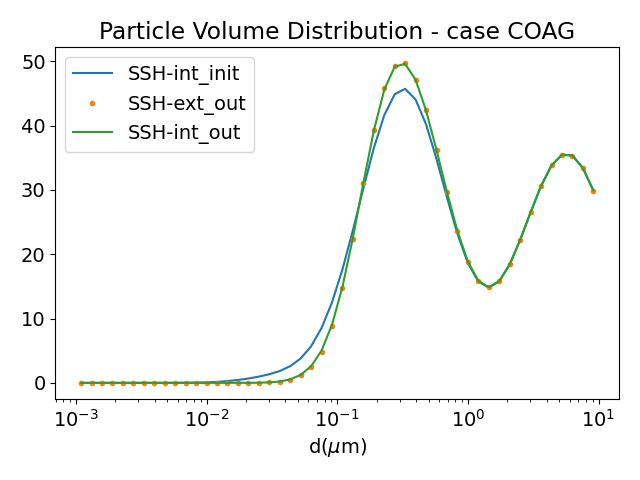
\includegraphics[angle=0,width=0.45\textwidth]{../graph/figure_ref/dVdlogd_COAG_EXT.png}
        \end{center}
\caption{Coagulation test case with mixing-state modelling. Number (left panel) and volume (right panel) concentrations.}
\label{fig-coag-ext}
\end{figure}
 
\begin{figure}[H]
        \begin{center}
                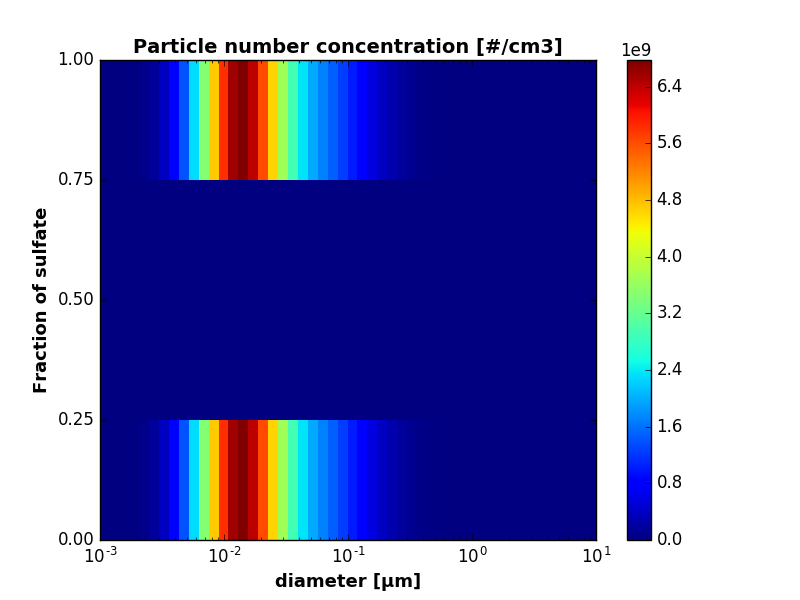
\includegraphics[angle=0,width=0.45\textwidth]{../graph/figure_ref/coag_ext_init.png}
                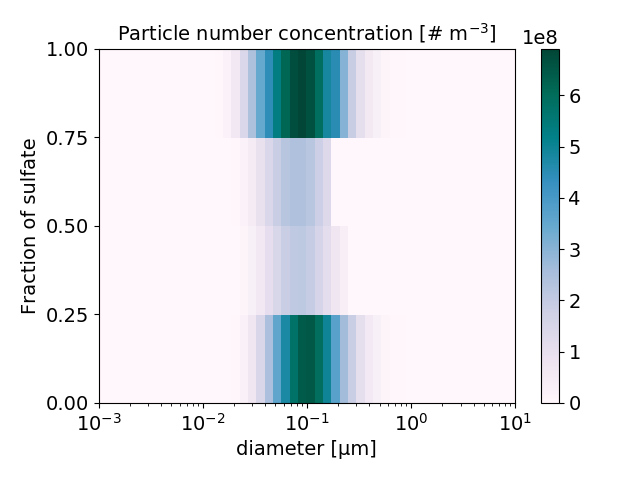
\includegraphics[angle=0,width=0.45\textwidth]{../graph/figure_ref/coag_ext_out.png}
        \end{center}
\caption{Number concentrations as a function of the size and fraction of one of the
two compounds at initial time (left panel) and after 12 h of simulation (right panel).}
\label{fig-coag-extb}
\end{figure}
 
\subsubsection{Condensation}

The effect of 
condensation on the mixing state is assessed by revisiting the condensation
test case (typical of a regional haze scenario, see section~\ref{cond-sulf}) by assuming
that the initial aerosol distribution is made of two low-volatility compounds
of same density (sulfate and another low-volatility compound).
As in \cite{zhu2015size}, 10 composition fractions are used.
The configuration file for this test is {\it{namelist\_cond\_ext.ssh}}.
Run the simulation by typing {\it{ssh-aerosol INIT/namelist\_cond\_ext.ssh}}.
By summing the mass and number of particles of all size fraction sections, the
size number and volume distribution are identical to those obtained with the
internal mixing assumptions. This can be checked by going to the repertory
{\it{graph}} and by running the python script {\it{dN\_Vdlogd\_cond\_ext.py}}
(see Fig~\ref{fig-cond-ext}).
The evolution of the mixing-state of particles after 12 h of condensation and coagulation may
be seen by comparing the two panels in Fig~\ref{fig-cond-extb}, which shows
the mass concentrations as a function of the size and fraction of one
sulfate, which is one of the
two compounds of the particles. 
Sulfuric acid condenses to form
sulfate. Because the condensation rate is greater for particles of
low diameters, the sulfate fraction is greater for those particles at the end
of the simulation (Figure~\ref{fig-cond-extb}).


\begin{figure}[H]
        \begin{center}
                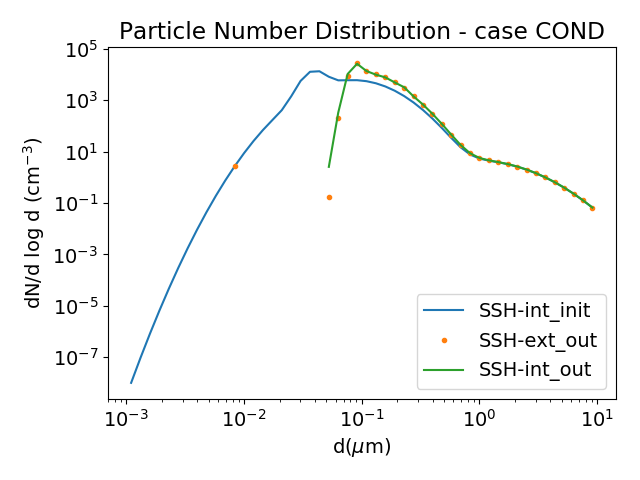
\includegraphics[angle=0,width=0.45\textwidth]{../graph/figure_ref/dNdlogd_COND_EXT.png}
                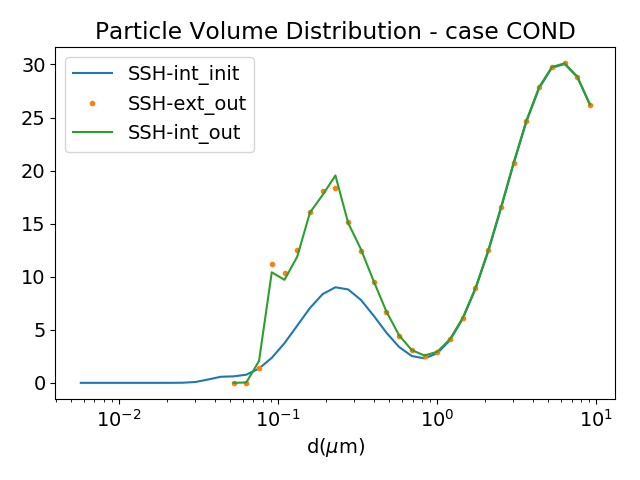
\includegraphics[angle=0,width=0.45\textwidth]{../graph/figure_ref/dVdlogd_COND_EXT.png}
        \end{center}
\caption{Regional haze test case with mixing-state modelling. Number (left panel) and volume (right panel) concentrations.}
\label{fig-cond-ext}
\end{figure}
 
\begin{figure}[H]
        \begin{center}
                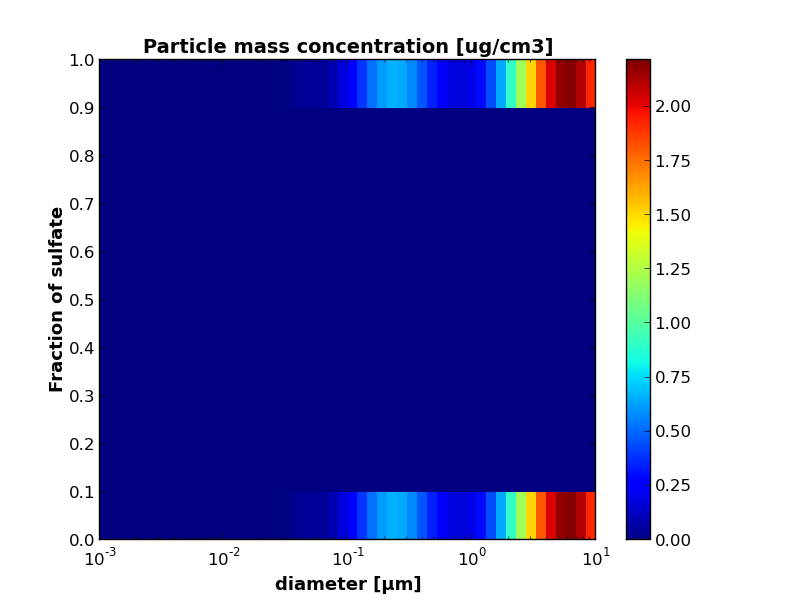
\includegraphics[angle=0,width=0.45\textwidth]{../graph/figure_ref/cond_mass_ext_init.png}
                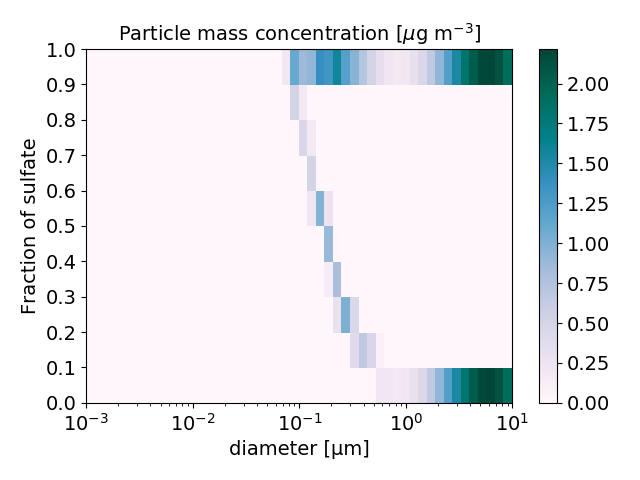
\includegraphics[angle=0,width=0.45\textwidth]{../graph/figure_ref/cond_mass_ext_out.png}
        \end{center}
\caption{Mass concentrations as a function of the size and fraction of one of the
two compounds at initial time (left panel) and after 12 h of simulation (right panel).}
\label{fig-cond-extb}
\end{figure}
 

\bigskip


\addcontentsline{toc}{section}{References}
\bibliographystyle{apalike}
\bibliography{testcases}

\end{document}
